Although I have not seen or read about the requirements of this document\footnote{So I still 
don't know how long it's supposed to be.}, through 
discussions with senior graduate students I've decided to include a preliminary `thesis 
schedule' in Sect.~\ref{sect:schedule} 
along with summaries of my thesis related work done to-date and what I'd like 
to do in the years following my graduate work.

\section{Things that I've done so far} \label{sect:donesofar}
My thesis related work done up until now has been dedicated to the modelling of RV 
timeseries with the inclusion of stellar jitter from the models discussed in 
Sect.~\ref{sect:jittermodels}. I've also developed the code necessary to implement the 
Gaussian process (GP) formalism of Sect.~\ref{chp:gp} to detecting planets in simulated 
RV timeseries using photometry and/or the Bisector inverse slope spectroscopic 
indicator to train the GP. \\

\subsection{RV detection of additional planets in transiting systems around inactive M-dwarfs}
These techniques were recently applied to a suite of simulated planetary systems around 
the slowly rotating (relatively inactive) M-dwarf GJ 1132 (Cloutier et al. \emph{in prep.}). 
The aim of this study was to compute the detection completeness 
of additional small planets in a fiducial planetary system consisting of a slowly rotating 
(inactive) M-dwarf with at least one known transiting planet. Such systems ($\sim 280$ 
of them) 
are expected to be discovered with the upcoming \emph{TESS} mission for which our 
results are applicable when RV follow-up observations of these systems are conducted. \\

Some important conclusions from this work are summarized below.

\begin{enumerate}
\item GJ 1132's light curve is modelled with a quasi-periodic GP which is then used to 
compute the corresponding RV jitter from active regions via the FF$'$ method. From this 
modelling we refine the stellar rotation period to be $122.31^{+6.03}_{-5.04}$ days. This value 
is consistent with the estimate of $\sim 125$ days obtained by assuming a purely sinusoidal 
model \parencite[no reported measurement uncertainty;][]{berta15}. The light curve in 
Fig.~\ref{fig:gj1132lc} is clearly not sinusoidal as the amplitude of the star's photometric 
variability appears to decrease over a few rotation cycles.  
\item Due to the star's small \vsini{,} the RV jitter from active regions is dominated by 
the suppression 
of the convective blueshift and is at its maximum observed value when the star's observed 
photometric variability is at its maximum value. When the photometric amplitude decreases, 
so too does the RV jitter to amplitudes comparable to or 
less than the imposed RV measurement uncertainty of 
$\sigma_{\mathrm{RV}} = 1$ \mps{.} When the amplitude of the RV jitter 
is greater than $\sigma_{\mathrm{RV}}$, a GP 
trained on the photometry does an excellent job of reducing the RV rms to levels comparable to 
$\sigma_{\mathrm{RV}}$ (Fig.~\ref{fig:gj1132gp}).
\item Using the occurrence rates of small planets around M-dwarfs, we compute the detection 
completeness of additional planets (planets not seen in transit) 
in slowly rotating M-dwarf transiting planetary systems. The results 
for the full sample are shown Fig.~\ref{fig:gj1132dc} for various values of the RV measurement 
uncertainty $\sigma_{\mathrm{RV}}$. 
\end{enumerate}

\begin{figure}
\centering
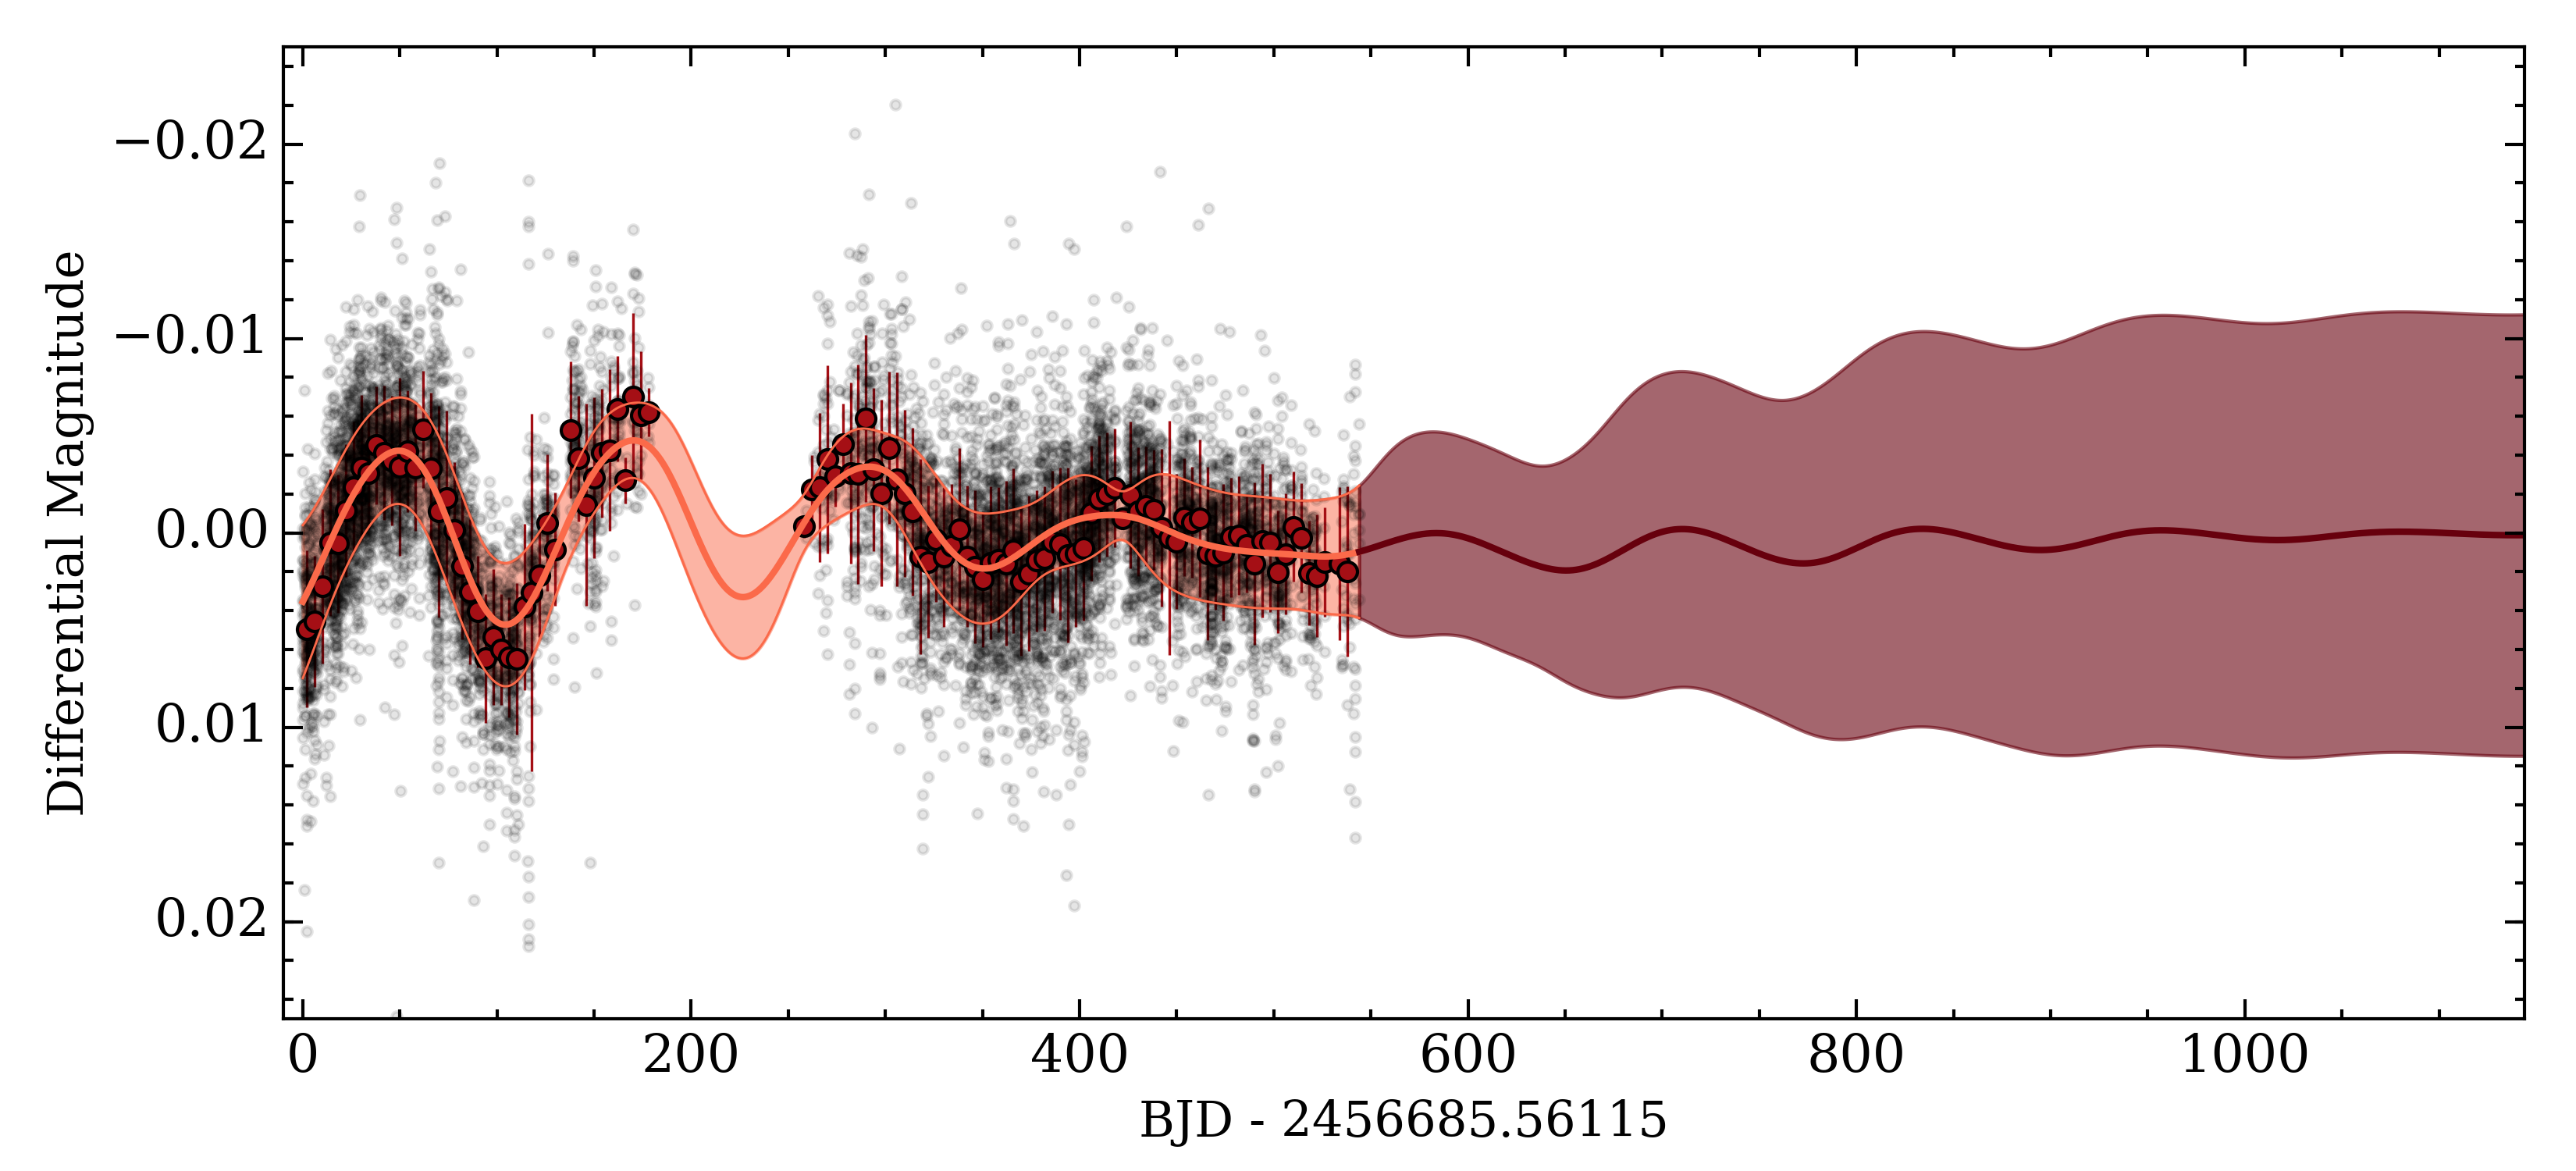
\includegraphics[scale=.55]{figures/gpmodel_testdummy_gponly.png}
\caption{The MEarth photometry originally presented in \cite{berta15}.
Red dots are the binned photometric measurements modelled with a
quasi-periodic Gaussian process (GP) which reveals a stellar rotation period of
$\sim 122$ days. The mean GP model and 99\% confidence
intervals are shown in pink. The GP predictive light curve and 99\%
confidence intervals are shown for 600 days following the last photometric
observation in red.
\label{fig:gj1132lc}}
\end{figure}

\begin{figure}
\centering
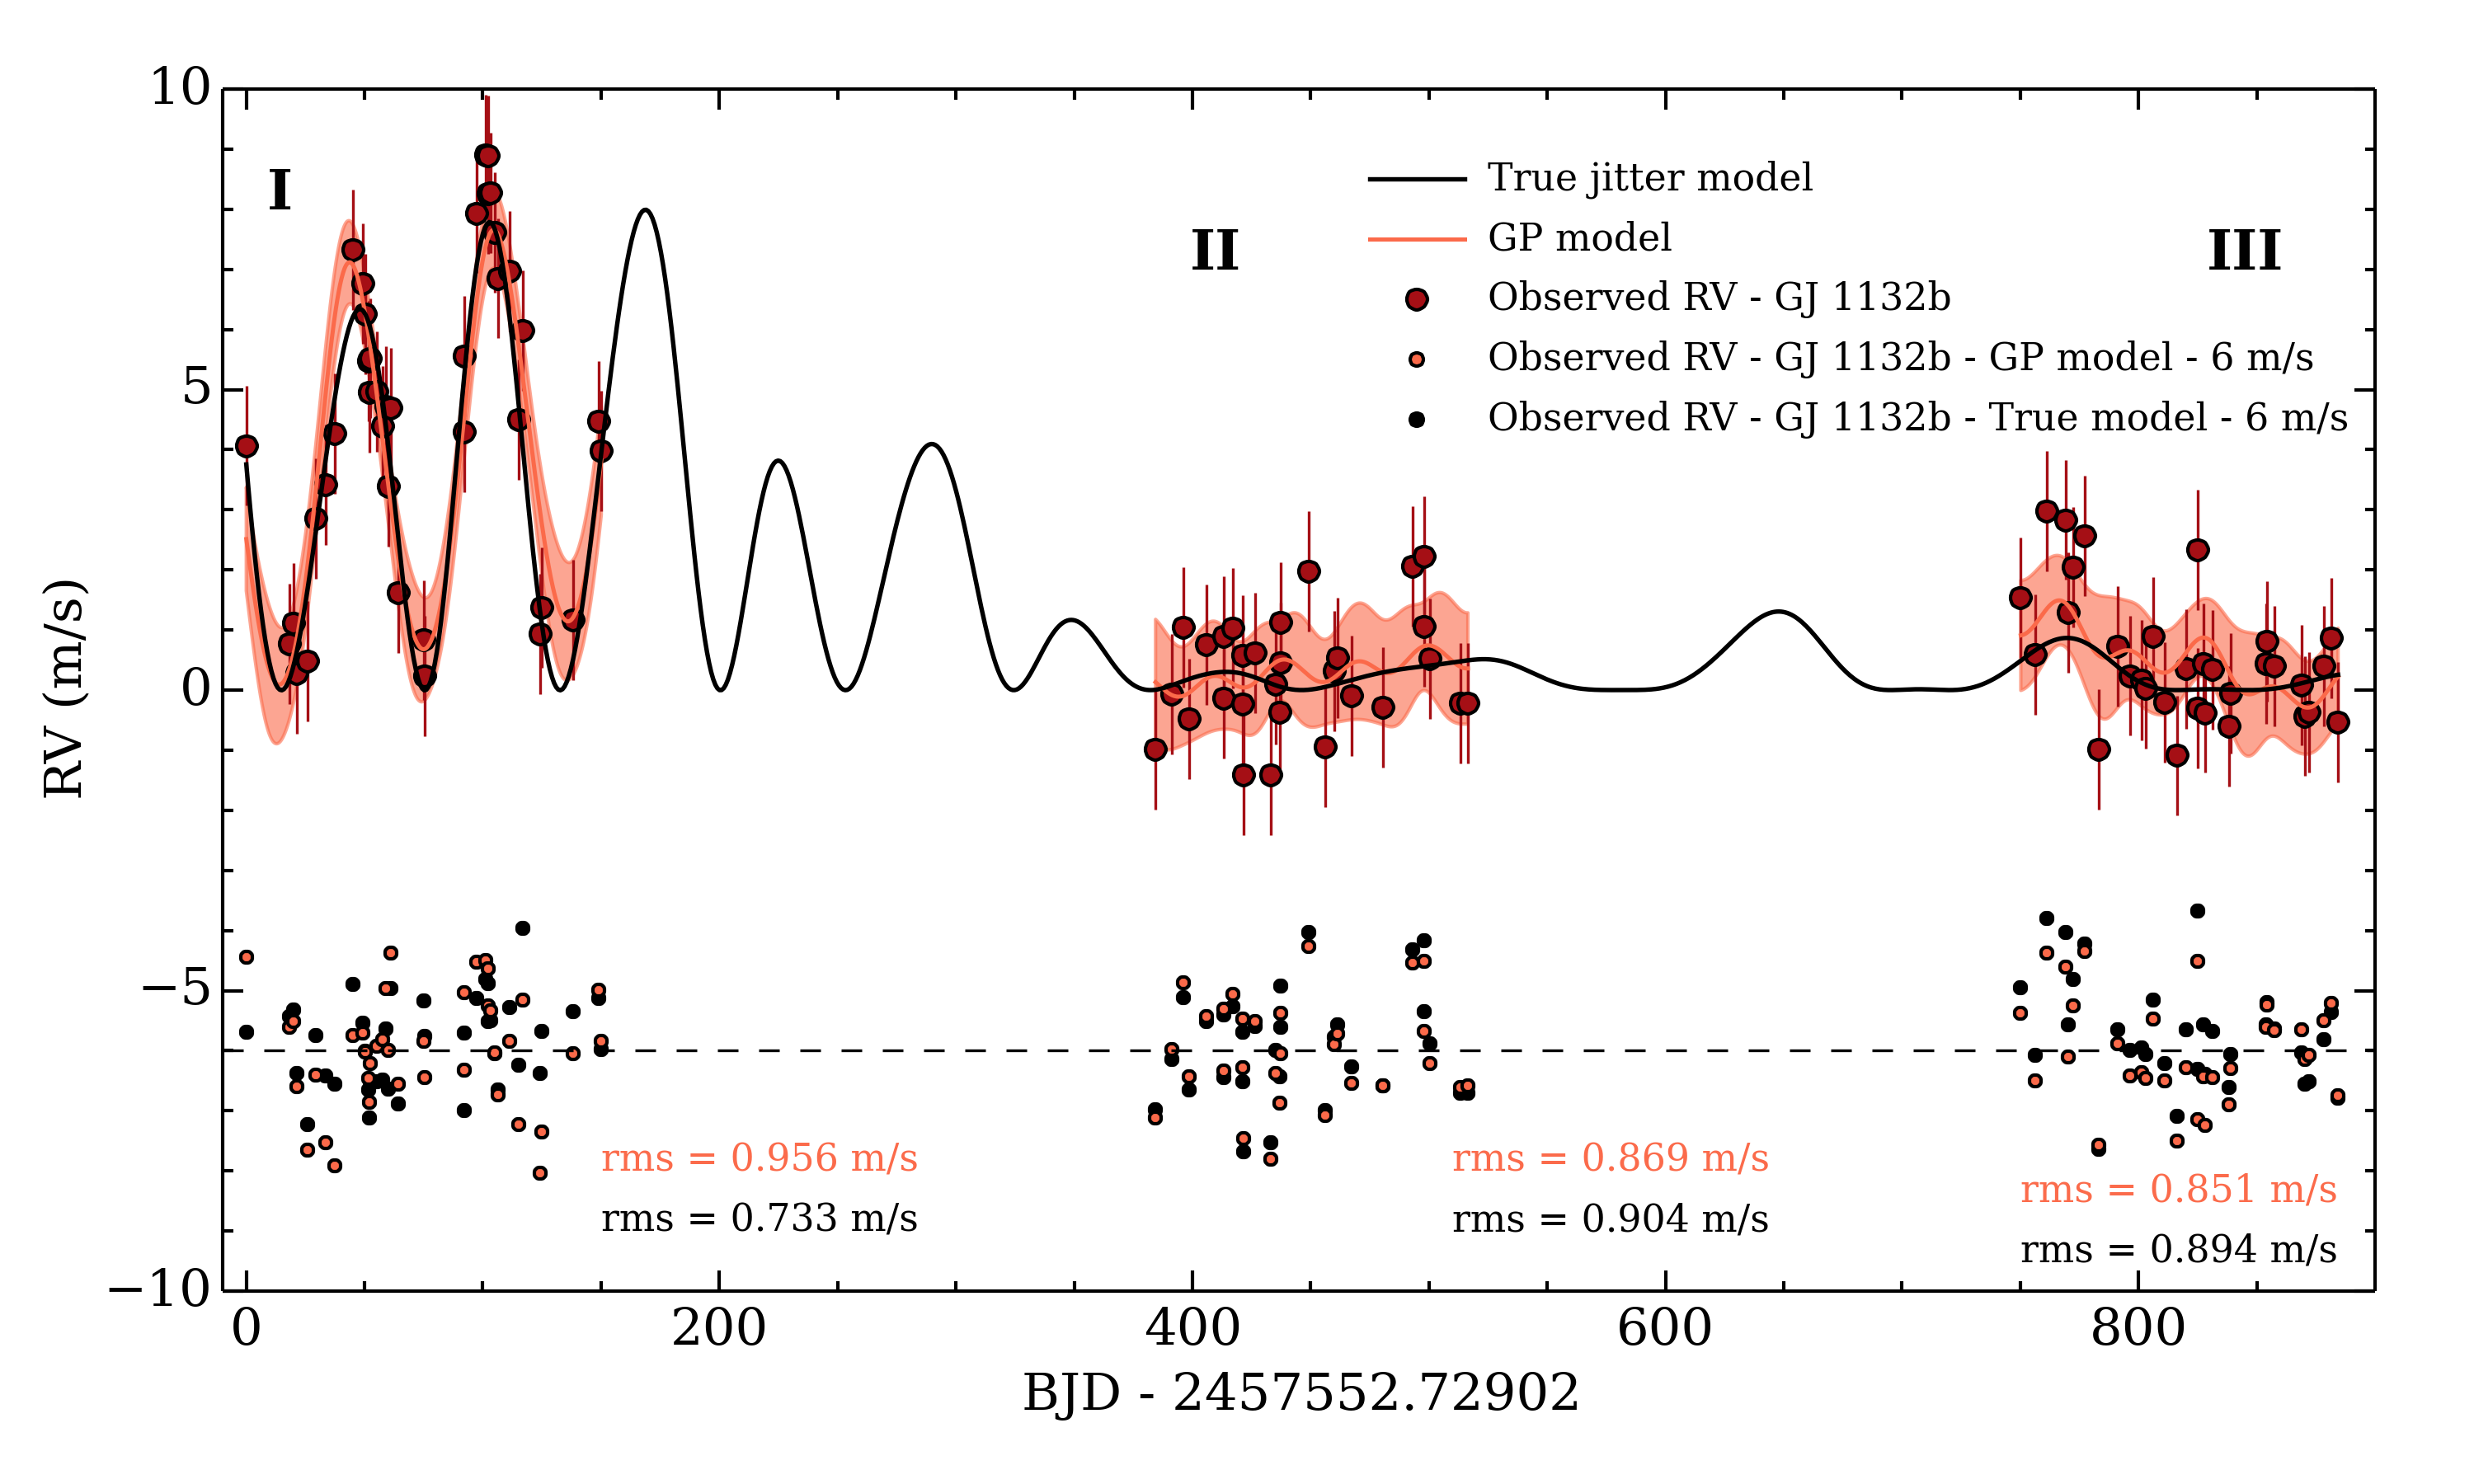
\includegraphics[scale=.55]{figures/GPjitter.png}
\caption{An example of a 1-planet simulated RV timeseries with the
keplarian contribution (from GJ 1132b) removed. The RV measurements (red
circles) therefore contain stellar jitter, predominantly from the suppression of
convective blueshift, and noise. The true jitter model from which the data are
derived is shown in black. The optimized quasi-periodic GP model and 95\%
confidence intervals for each observing window (I,II,III) are shown in pink.
The shifted residuals about the true model are plotted as black points while the
shifted residuals about the
GP model are plotted as pink points. The rms of each set of residuals is
annotated in the panel (true model residuals and GP model residuals in black and
pink respectively). 
\label{fig:gj1132gp}}
\end{figure}

\begin{figure}
\centering
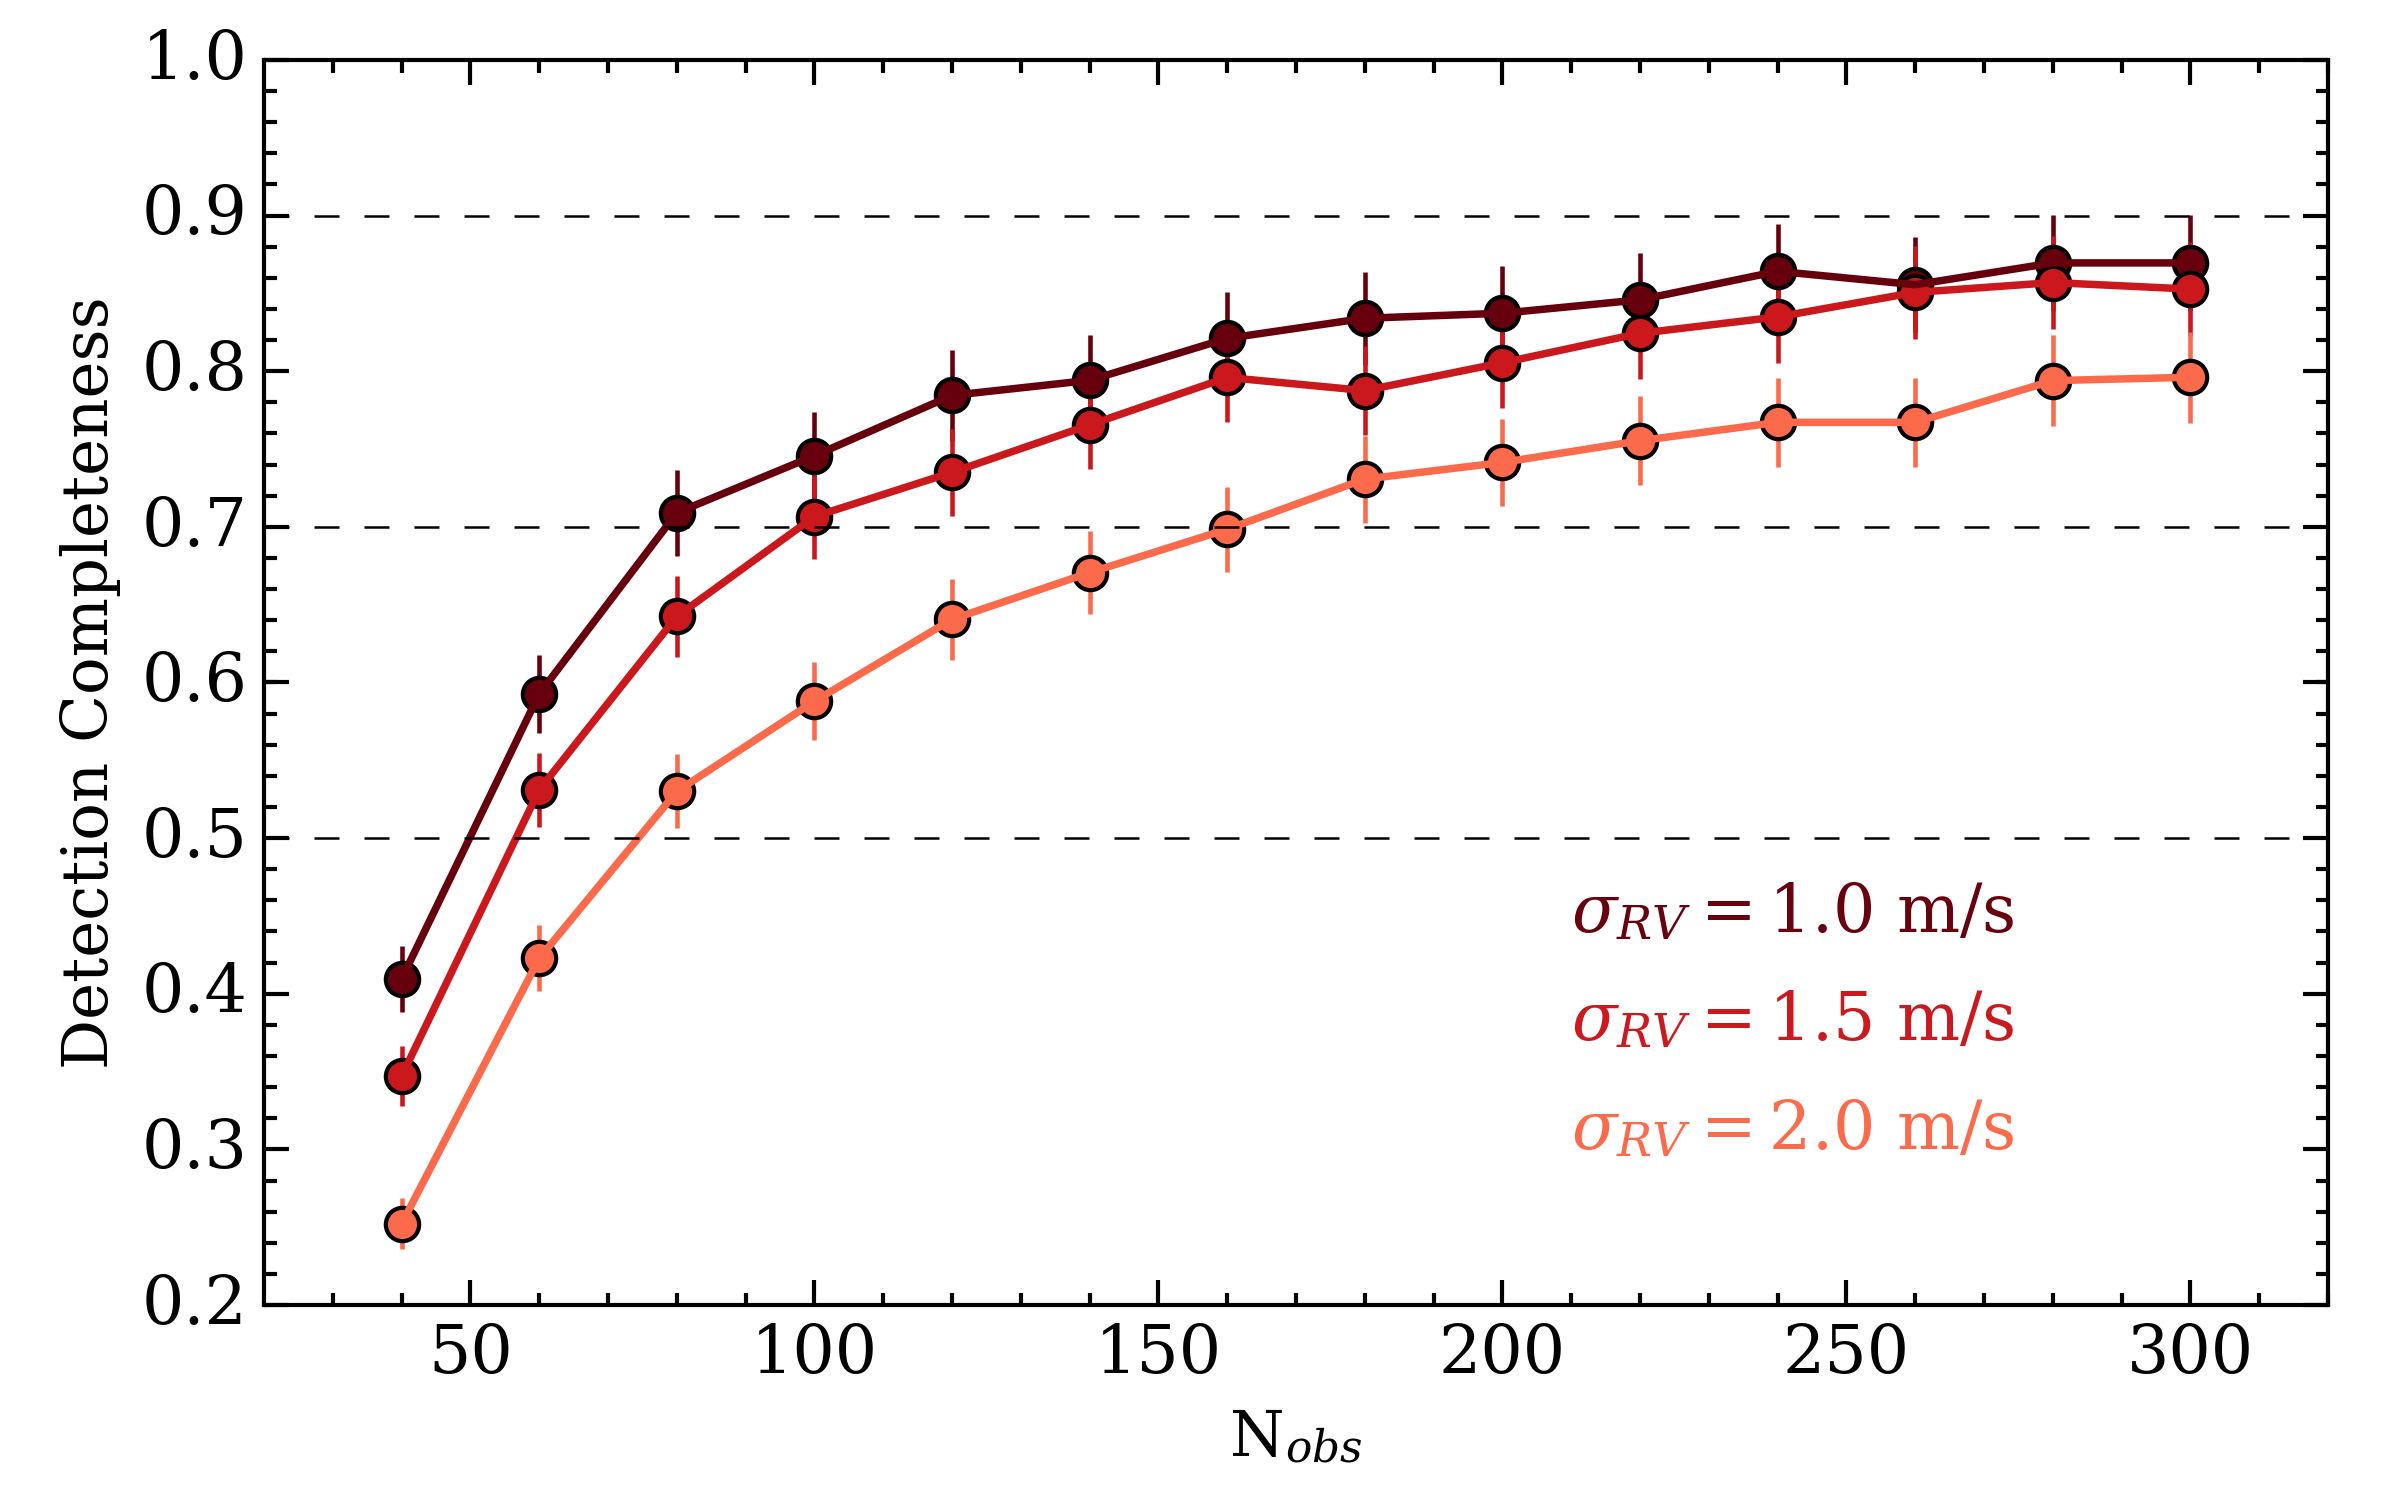
\includegraphics[scale=.6]{figures/detfreq.png}
\caption{The detection completeness for the entire sample of additional planets
around GJ 1132 for various values of the RV measurement error. Errorbars are
from Poisson statistics. Dashed
horizontal lines at 50, 70, and 90 per cent completeness are included to guide the eye. 
\label{fig:gj1132dc}}
\end{figure}

\subsection{Detection of the Rossiter-McLaughlin effect from small planets}
A simplified version of the code used on GJ 1132 was applied to the TRAPPIST-1 
multi-planetary system around a rapidly rotating ultracool dwarf \parencite{gillon16}. 
This system represents a superlative opportunity to measure the Rossiter-McLaughlin (RM) 
effect from a small (likely rocky) transiting planet. The RM effect is an anomalous 
RV signal seen when a planet transits its host star. Similar to the flux effect from 
active regions, as the planet occults the opposing limbs of the stellar disk an 
anomalous Doppler shift is observed causing a bump in the RV timeseries within the 
planet's transit window. The observed RM waveform is dependent on the transiting planet's 
trajectory across the stellar disk and can therefore be used to measure the 
projected spin--orbit angle $\beta$ of the normal to the planet's orbital plane and the 
stellar spin axis. For reference, $\beta=0^{\circ}$ for perfectly aligned systems, 
$\beta=90^{\circ}$ for perfectly misaligned systems, and $\beta=180^{\circ}$ for aligned systems 
which are retrograde. 
To date, the RM effect has only been detected for giant planets. 
Fig.~\ref{fig:rm} shows an example of this for the hot Jupiter HD 189733b whose 
projected spin--orbit angle is $\beta < 1^{\circ}$. \\

\begin{figure*}
\centering
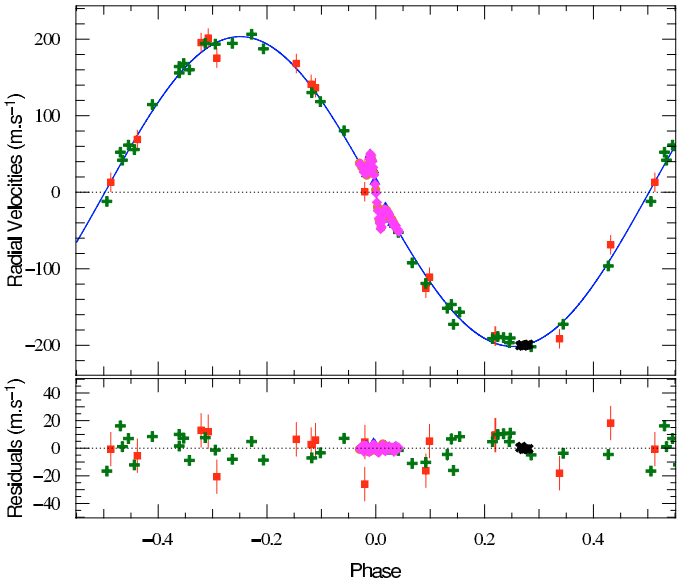
\includegraphics[scale=.3]{figures/hd189733rm1.png}
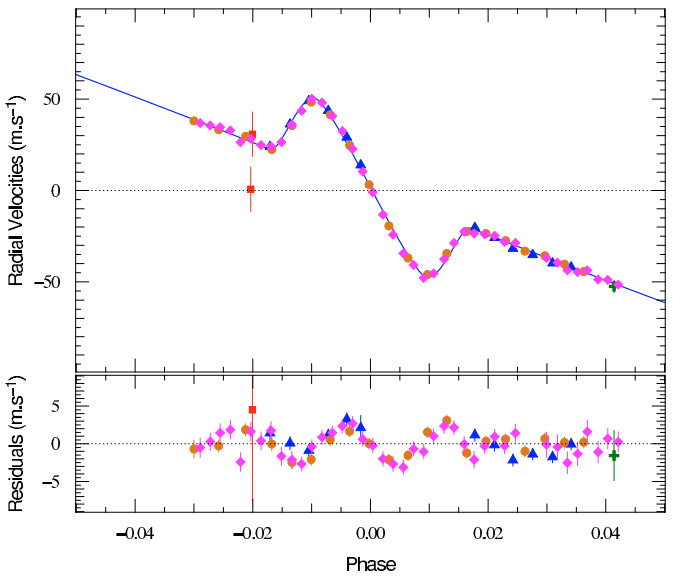
\includegraphics[scale=.3]{figures/hd189733rm2.png}
\caption{\emph{Left panel}: the phase-folded RV timeseries for the hot Jupiter 
HD 189733b. \emph{Right panel}: zoom-in on the transit window to reveal the anomalous 
RM effect. \parencite[Image credit:][]{triaud09} \label{fig:rm}}
\end{figure*}

The amplitude of the RM effect is 

\begin{equation}
K_{\mathrm{RM}} = v\sin{i_s} \frac{D}{1-D},
\end{equation}

\noindent where $D=(r_p/R_s)^2$ is the transit depth \parencite{gaudi07}. 
Detection of the RM effect for a planet of a given size therefore favours a small host 
star which is rapidly rotating such as TRAPPIST-1. Taking the TRAPPIST-1 system as a 
fiducial test case, a suite of RV timeseries with the RM effect are used to compute the 
measurement accuracy of the spin--orbit angle $\beta$ for small planets. 
Fig.~\ref{fig:beta} from Cloutier et al. \emph{submitted} shows the accuracy with which 
$\beta$ can be measured in an RV timeseries. 
Fig.~\ref{fig:KrmKdop}, also from Cloutier et al. \emph{submitted}, shows the relative 
Doppler semiamplitude and RM semiamplitude of a habitable zone Earth-twin along with the 
population of nearby and Kepler field M-dwarfs in the \vsini{}, $M_s$ plane. There clearly 
exists a large subset of M-dwarfs for which the RM semiamplitude is large compared to the 
Doppler semiamplitude and therefore represent optimal targets for characterizing the 
distribution of small planet spin--orbit angles, an important quantity for probing the 
orbital history of a planetary system since well-aligned systems are predicted from 
models of terrestrial planet formation and highly misaligned system may be reconciled with 
past dynamical events such as planet-planet interactions 
\parencite{rasio96, weidenschilling96} or Kozai migration \parencite{wu03}. \\

\begin{figure}
\centering
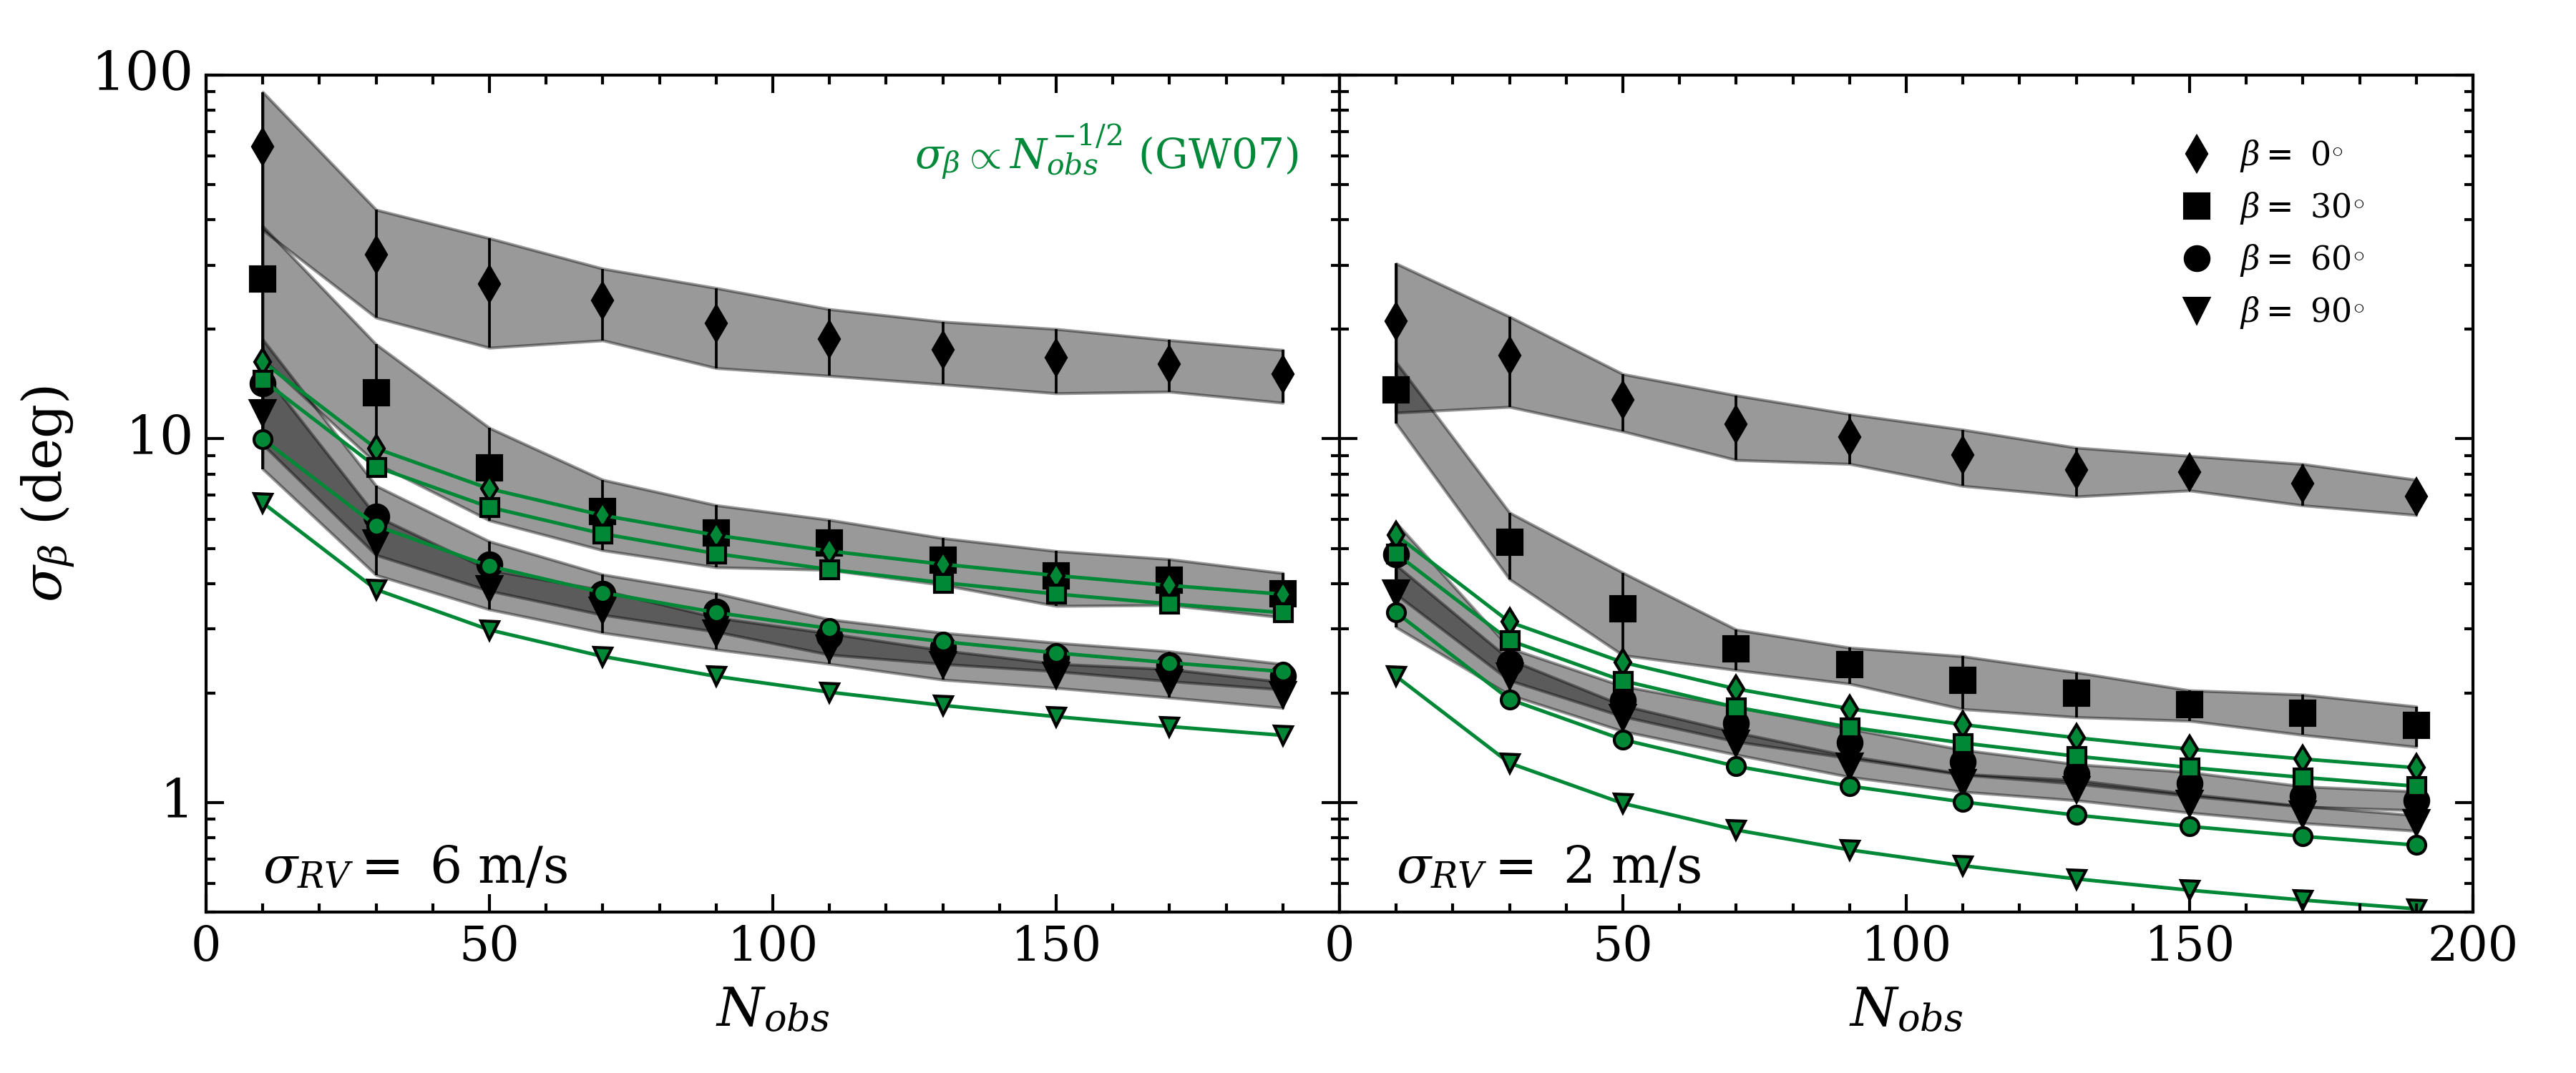
\includegraphics[scale=.5]{figures/betaerr3_trappist1.png}
\caption{The average measurement uncertainty of the spin--orbit angle for the two innermost 
TRAPPIST-1 planets 
from the measurement of the Rossiter-McLaughlin waveform as a function of the number of
RV measurements made in-transit. Values of
$\beta=0^{\circ},30^{\circ},60^{\circ},90^{\circ}$ are considered for both
cases of the RV measurement uncertainties ($\sigma_{\mathrm{RV}}=6$
\mps{;} \emph{left} and $\sigma_{\mathrm{RV}}=2$ \mps{;} \emph{right}). The shaded regions
approximately depict the $1 \sigma$ confidence intervals from the dispersion in $\sigma_{\beta}$ after
multiple Monte-Carlo realizations. The \emph{green curves} represent
the predicted measurement uncertainty from \cite{gaudi07}. 
\label{fig:beta}}
\end{figure}

\begin{figure}
\centering
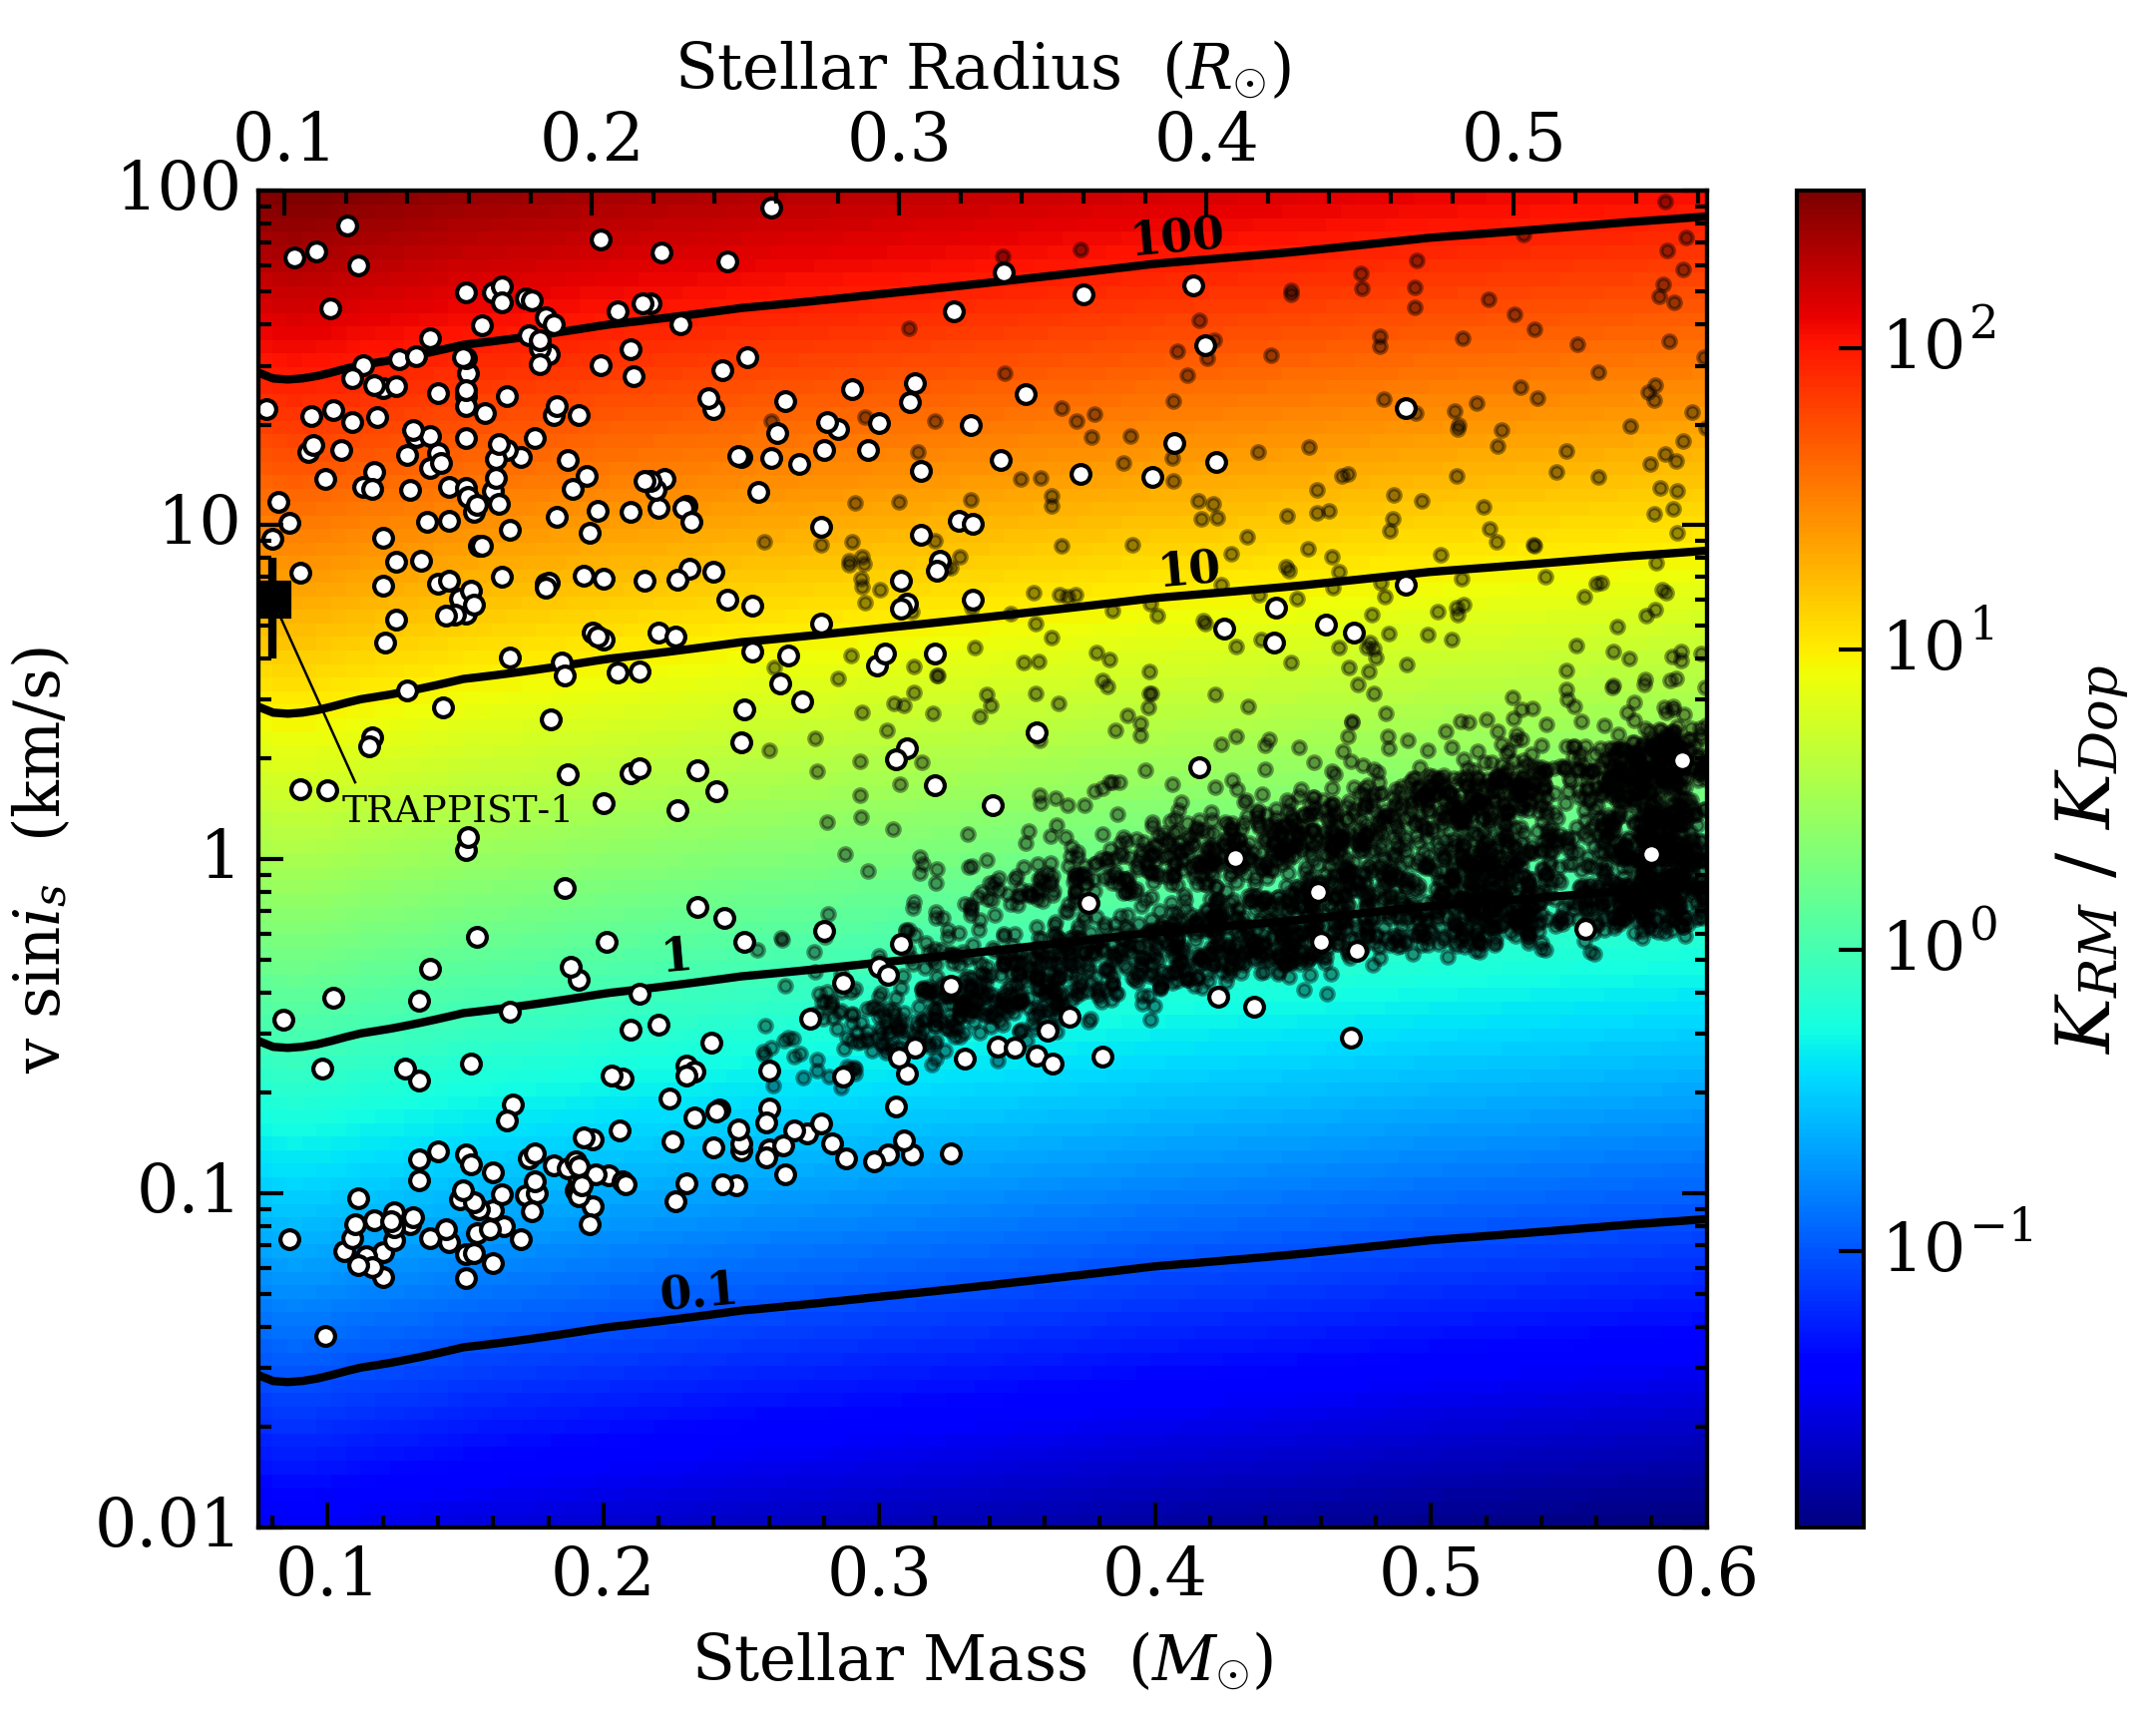
\includegraphics[scale=.5]{figures/Krm_Krv.png}
\caption{The ratio of the Rossiter-McLaughlin semiamplitude to the Doppler
semiamplitude for an Earth-sized planet at the
inner edge of the habitable zone. \emph{White} and \emph{black}
symbols depict stellar rotation periods measured with MEarth
\parencite{irwin11, newton16a} and Kepler \parencite{mcquillan14} respectively.
TRAPPIST-1 is depicted as the \emph{black square} according to its mass.
Over the range of
observed M-dwarf rotation velocities, the semiamplitude of the
RM effect can be over two orders-of-magnitude less than or greater than
the Doppler semiamplitude of a typical rocky planet in the habitable zone. 
\label{fig:KrmKdop}}
\end{figure}


\section{Thesis Schedule: things that I propose to do} \label{sect:schedule}
\subsection{Planet yield simulations: \spirou{} legacy survey \& \emph{TESS}}   
The most imperative upcoming tasks involve calculations similar to those done 
specifically for the class of slowly rotating M-dwarf transiting planetary systems. 
Namely, to investigate the observational effort required to i) characterize transiting 
planet candidates to a desired accuracy and ii) to detect exoplanets in 
a blind fashion such as what will be done in the \spirou{} legacy survey. These 
calculations are necessary when applying for telescope time and dividing the total 
time allocation among the instruments' various science campaigns (i.e. exoplanet 
detection/characterization versus star formation). I am currently in the process of 
performing these calculations based on the i) projected sample of \emph{TESS} candidate 
systems \parencite{sullivan15} 
and ii) the sample of 100 closest M-dwarfs in the Northern sky populated with 
planets based on the occurrence rates derived from Kepler \parencite{dressing15a}. 
These calculations also offer testbeds of the GP formalism for modelling stellar 
jitter because the RV timeseries are synthetic implying that we know the input 
jitter model 
which we can compare to the GP models to monitor its performance. \\

Each of the aforementioned calculations requires a large suite of simulated RV timeseries 
with a variety of stellar (e.g. $M_s, P_{\mathrm{rot}}$, etc.) and planetary parameters 
(e.g. $P,K$, planet multiplicity, etc.). At the end of the day, the interesting quantity 
is similar to what is shown in Fig.~\ref{fig:gj1132dc}: the detection completeness 
as a function of the number of RV measurements \nobs{.} 
Although in the case of a blind survey, 
this quantity will be marginalized over the stellar and planetary parameters. Whereas 
for the 
mass characterization of transiting planet candidates, another quantity of interest is 
the mass detection significance as a function of \nobs{,} which will be marginalized over 
the stellar parameters only given that the planetary parameters are unique to each 
system and are reported in \cite{sullivan15}. \\

\emph{Preliminary} results from the latter calculation will not be discussed here but 
I can comment further on the apparent effectiveness of GPs at mitigating the effects of 
stellar jitter and characterizing the semiamplitudes of the \emph{TESS} planet candidates. 
Fig.~\ref{fig:gpcomp} compares the input RV jitter model with the predicted quasi-periodic 
GP jitter model. This is one of the \emph{TESS} candidate systems with a potentially 
habitable transiting planet ($M_s=0.2$ M$_{\odot}$, $T_{\mathrm{eff}}=3300$ K, $P_{\mathrm{rot}}=1.1$ 
days, $P=23.1$ days, $K=2.65$ \mps{)}. The rapid stellar rotation makes the star an active 
one with 
a maximum RV jitter amplitude of $>20$ \mps{} or almost an order of magnitude greater than 
the planetary signal. It is apparent in Fig.~\ref{fig:gpcomp} 
that the GP model, plus a single keplarian mean function, is a good model of the RV jitter.
In this simulation the GP hyperparameters are trained on a BIS timeseries computed using 
the \texttt{SOAP 2.0} code (see Sect.\ref{sect:soap}). \\

\begin{figure}
\centering
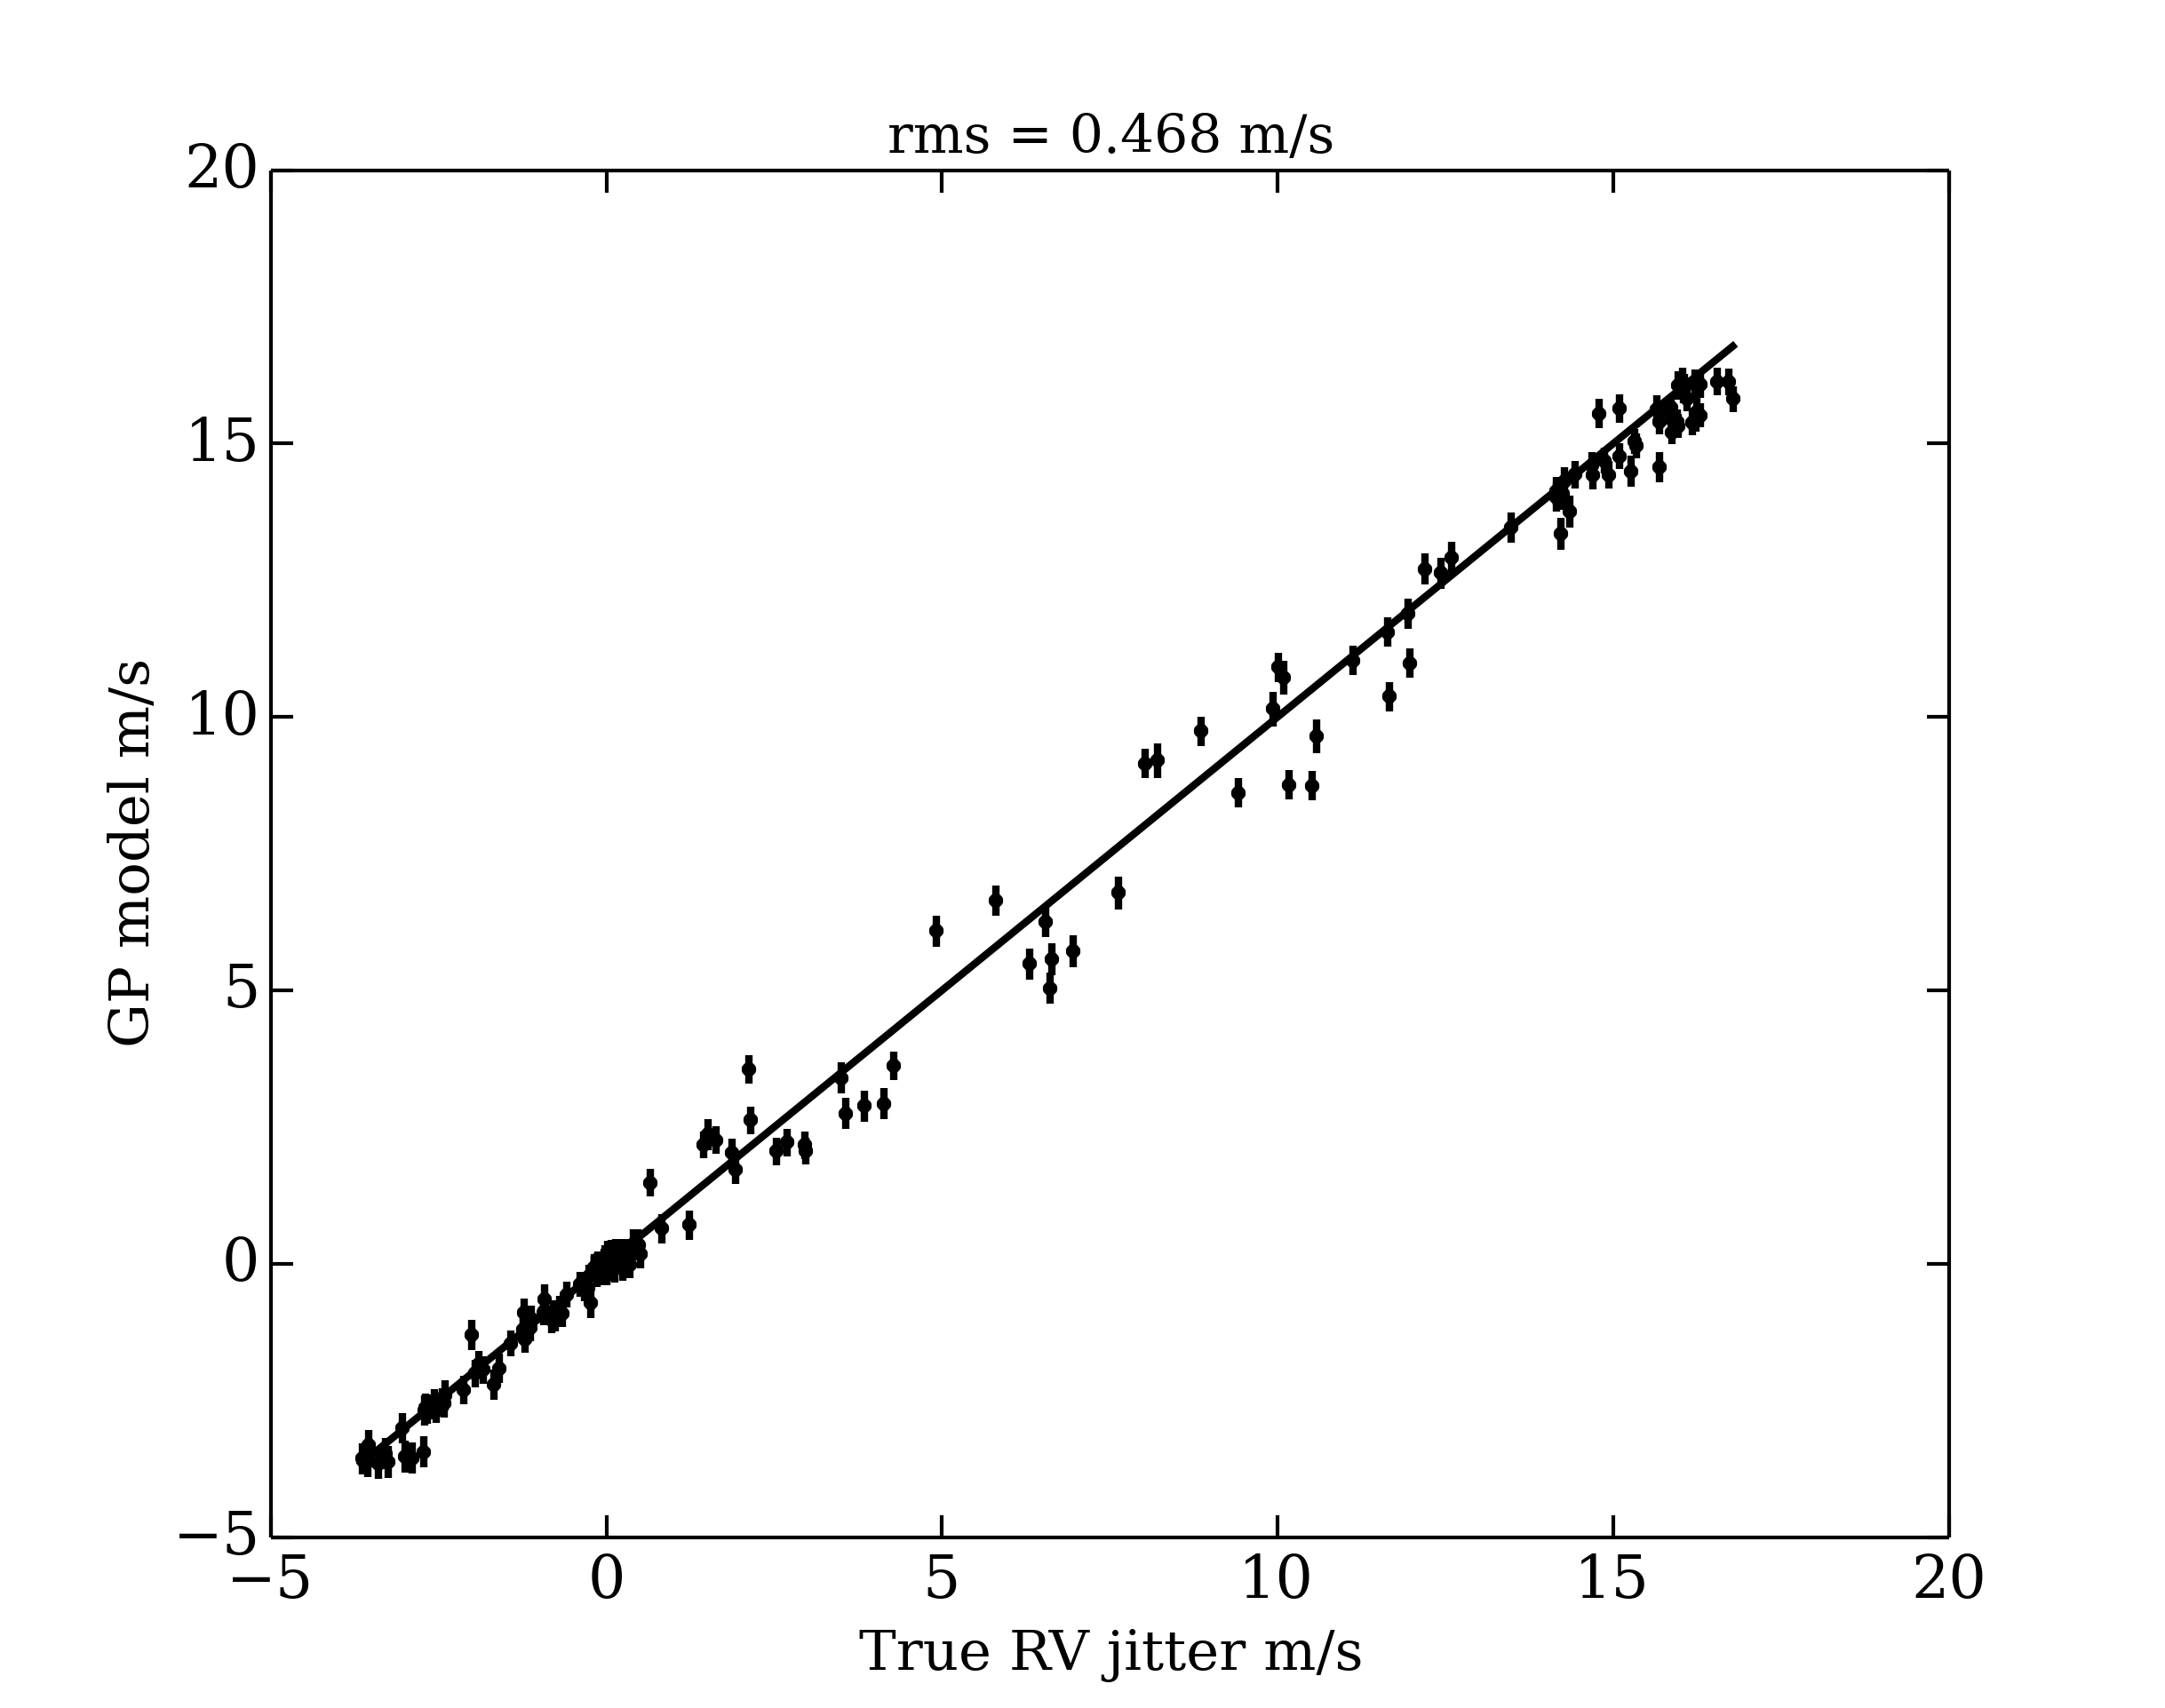
\includegraphics[scale=.5]{figures/gpcomparison.png}
\caption{Comparison of the input (\emph{true}) RV jitter model computed using the methods 
of Sect.~\ref{sect:jittermodels} with the predictive GP jitter model after removal of a 
single keplarian component. The rms of the residuals is sub-\mps{.}
\label{fig:gpcomp}}
\end{figure}

\subsection{GPs applied to real datasets}
The next step will still be prior to \spirou{'s} first light in 2018. 
It should involve moving away from synthetic data and instead applying the GP formalism 
to particular systems whose i) characterization will be improved by \spirou{} and/or 
ii) are 
attractive targets for atmospheric characterization with \emph{JWST}. An example of the 
former is the young hot Jupiter around the T-Tauri star V830 Tau \parencite{donati16}. 
The discovery paper constructs a RV activity timeseries from the Doppler imaging 
brightness image. A GP regression may be able to improve the modelling of the 
residual RVs and obtain a more accurate estimate of the planet properties. 
A candidate for atmospheric characterization, which requires an accurate mass measurement 
to infer physical properties of the atmosphere, is K2-18b \parencite{montet15}. K2-18b is 
a mini-Neptune sized planet in the habitable zone ($r_p = 2.24$ R$_{\oplus}$, $P=33$ days) 
of a nearby ($\sim 34$ pc) early-to-mid M-dwarf. 
The K2 light curve may be used to train a GP used for future RV 
modelling is conjunction with spectral indicators which will be obtained contemporaneously 
with RV measurements. This target has yet to have its mass characterized which is 
required in order to distinguish its bulk composition between a `water-world' and a rocky 
planet with an extended gaseous envelope. \\

\subsection{Application of other machine learning algorithms}
Following my work with GPs, I've also delved into the world of machine learning (ML) algorithms 
with the prospect of applying them to my research. The investigation of these algorithms 
has also been facilitated by the 
handful of ML workshops hosted by postdocs and faculty at the Centre for Planetary Sciences. 
As an example, a number of researchers attending these workshops are attempting to use 
an optimized classification algorithm to detect planetary transits in a stellar light curve 
from missions like \emph{TESS}. Preliminary results on this front have been impressive. 
That is that in synthetic light curves, transiting planets are recovered with a $>90$\% 
detection efficiency. 
My hope is to extend this work to the detection of planets in RV timeseries although the 
details of doing so have yet to be worked out. \\

On a shorter timescale, ML regression algorithms may be applicable to the datasets generated 
from my Monte-Carlo simulations for the \spirou{} legacy survey and \emph{TESS} candidates. 
As an example in the latter case, consider a newly discovered \emph{TESS} transiting planet 
candidate with a known orbital period $P$ and planet radius $r_p$ around a star 
with a stellar mass estimate $M_s$ and rotation period $P_{\mathrm{rot}}$ measured from its 
light curve. Using a statistical planetary mass-radius relationship 
\parencite[e.g.][]{lopez14, weiss14, wolfgang16} and the values of $P$ and $M_s$, we can 
estimate the expected RV semiamplitude $K$ (see Eq.~\ref{eq:K2}) which is undoubtedly an 
important feature when estimating i) the number of observations required to detect the planet 
with RV measurements \nobs{} and ii) the detection significance of the RV semiamplitude and 
hence of the planet mass; $m_p/\sigma_{m_p}$. 
Using the extensive set of features\footnote{Some presumably important examples of features 
might be $M_s, P_{\mathrm{rot}}, \sigma_{\mathrm{RV}}, P, K$,etc.} 
and target values (\nobs{} 
and $m_p/\sigma_{m_p}$) generated by my Monte-Carlo simulations of the 
\emph{TESS} planet candidate RVs, can we train a ML regression model to predict either 
target value for an input set of features pertaining to a unique \emph{TESS} system? 
The answer 
will be investigated soon given the importance of prioritizing \spirou{} follow-up 
observations of \emph{TESS} candidates as these will likely be the first science cases 
that \spirou{} focuses on following its first light. The importance of the mass characterization 
of transiting planet candidates is emphasized by the approaching launch date of \emph{JWST} 
and its unique ability to characterize the atmospheres of transiting planets. 

\subsection{Transiting planets with \spirou{}}
Given the proximity of \spirou{'}s first light and the tentative completion date of my thesis, 
my first \spirou{} science cases will likely involve transiting planet characterization rather than 
exoplanet discoveries. \emph{Such studies will represent the culmination of most of my work up until 
that point with the use of GPs to fit the planetary signal in RV and measure the planet's 
mass and orbit}. Certain transiting planets may also have a measurable Rossiter-McLaughlin effect 
which may be characterized during the RV follow-up effort. \\

While we wait for \emph{TESS} and \spirou{,} time will be spent to develop and calibrate a 
\emph{merit function} to be used to prioritize transiting planet candidates. 
A number of obvious variables 
of the merit function will be the candidate's orbital period, expected RV semiamplitude, and 
near-IR apparent magnitude. Also to be included is the expected RV jitter from the host star 
which will heavily influence the our ability to detect planetary signals with \spirou{.}


\section{Things that I'd like to do but simply cannot do in 3 years} \label{sect:liketodo}
The first one is probably obvious to those that know me and that is to 
\emph{find a damn planet}. If a new exoplanet discovery is not on my CV in the 
next say, 4 years, then I'm going to be very disappointed and will likely have to 
re-evaluate my time management skills. Unfortunately, detecting a new exoplanet 
with \spirou{} before the end of my PhD is unrealistic given that the legacy survey, 
wherein new exoplanets will be detected, will not have progressed far enough for a 
sufficient number of observations over a sufficiently long time baseline 
to reasonably enable the detection of a planet in a `blind' 
manner. As an aside, one may then turn one's attention to the \emph{GAIA} satellite 
which will have yearly data releases starting on 
September 14th\footnote{Happy Birthday Mom!} of this year. 
\emph{GAIA} is projected to detect a cosmic s\%\$@-tonne of planets 
\parencite[$\sim 21$ 000;][]{perryman14} via the astrometry method whose timeseries 
modelling features many similarities with RV fitting. \\

As mentioned in Sect.\ref{sect:survey}, \spirou{} will conduct of survey of 
nearby M-dwarfs in the Northern sky and undoubtedly detect a population of planets 
around the coolest class of dwarf star; mid-to-late M-dwarfs. The conclusion of 
the 5-year long survey will allow us to compute the previously unexplored planet 
occurrence 
rates around these cool stars and the value of $\eta_{\oplus}$\footnote{$\eta_{\oplus}=$ 
the fraction of stars 
which host an Earth-like planet in its habitable zone.} down to the lowest stellar 
masses. I'd like to make this calculation. The problem itself is extremely 
interesting scientifically and the steps involved in making the calculation will fall 
right into my areas of expertise. The problem's got it all: 
RV data analysis (which includes jitter modelling), planet detection, 
and astrostatistics! Happy days.

\section{Point-form Thesis: Thesis Proposal}
\begin{itemize}
\renewcommand\labelitemi{--}
\item~\ref{sect:donesofar} \textbf{Things that I've done so far}: created synthetic radial velocity timeseries 
including planetary companions, instrumental noise, and stellar jitter and computed 
\begin{itemize}
\item the detection completeness of non-transiting planets around slowly rotating M-dwarfs with 
at least one known transiting planet, and
\item the accuracy with which we can measure the projected spin--orbit angle of rocky planets 
around M-dwarfs via the Rossiter-McLaughlin effect.
\end{itemize}
\item~\ref{sect:schedule} \textbf{Thesis Schedule: things that I proposed to do}: 
\begin{itemize}
\item continue to use synthetic radial velocity timeseries to compute the exoplanet detection yield 
of the \spirou{} legacy survey and of transiting candidates with radial velocity follow-up observations,
\item apply Gaussian process regression to model radial velocity jitter and further characterize 
existing planetary systems, 
\item develop machine learning algorithms for model fitting and possibly to the `blind' detection 
of new exoplanets in radial velocity data, and
\item characterize transiting planets with \spirou{.}
\end{itemize}
\item~\ref{sect:liketodo} \textbf{Things that I'd like to do but simply cannot in do in 3 years}: 
\begin{itemize}
\item \emph{discover a new exoplanet} 
in radial velocity with \spirou{} or jump on the \emph{GAIA} bandwagon 
and do it via astrometric measurements, and
\item compute the frequency of habitable zone Earth-like planets around the latest stars at the 
end of the \spirou{} legacy survey.
\end{itemize} 
\end{itemize}
